% =====================================================================
%  Grace et al. 2024 — "Thousands of AI Authors on the Future of AI"
%  Executive slide deck — built around four "wait-WHAT" moments.
% =====================================================================
\documentclass[aspectratio=169, 12pt, xcolor={dvipsnames,table}]{beamer}
\usetheme{metropolis}
\usepackage{tikz}
\usepackage{graphicx}
\usepackage{booktabs}
\usepackage{appendixnumberbeamer}

% Tighter metropolis tweaks
\setbeamerfont{title}{size=\Large, series=\bfseries}
\setbeamerfont{frametitle}{size=\large, series=\bfseries}
\metroset{progressbar=frametitle, sectionpage=progressbar, numbering=fraction}

\definecolor{accent}{HTML}{B02418}
\definecolor{ink}{HTML}{1A1A1A}
\definecolor{mute}{HTML}{888888}

\newcommand{\bignum}[1]{{\fontsize{60}{66}\selectfont\bfseries\color{accent}#1}}
\newcommand{\midnum}[1]{{\fontsize{36}{40}\selectfont\bfseries\color{accent}#1}}
\newcommand{\whatmoment}[1]{%
  \begin{frame}[plain]
    \centering
    \vfill
    {\color{mute}\large wait ---}\\[0.6em]
    {\fontsize{48}{52}\selectfont\bfseries\color{accent} WHAT?}\\[1.2em]
    {\Large #1}
    \vfill
  \end{frame}}

\title{Thousands of AI Authors}
\subtitle{What 2,778 researchers actually think the next 20 years look like}
\author{\small after Grace, Stewart, Sandk\"uhler, Thomas, Weinstein-Raun, Brauner (2024)}
\date{}

\begin{document}

% ---------------------------------------------------------------
\begin{frame}[plain]
  \titlepage
\end{frame}

% ---------------------------------------------------------------
\begin{frame}{One survey. One question per expert.}
  \vfill
  \begin{columns}[T]
    \column{0.45\textwidth}
    \bignum{2{,}778}\\[0.4em]
    {\large AI researchers}\\
    {\small every NeurIPS, ICML, ICLR,\\JMLR, AAAI, IJCAI author\\from the previous year}
    \column{0.45\textwidth}
    \vspace{1.5em}
    {\large Asked in 2023.}\\[0.3em]
    {\large Same questions as 2022.}\\[1em]
    {\color{mute}Largest expert survey of its kind.\\Answers sealed before GPT-4 retail launch.}
  \end{columns}
  \vfill
\end{frame}

% ---------------------------------------------------------------
\begin{frame}[plain]
  \centering\vfill
  {\color{mute}\large The story of this paper is four moments.}\\[2em]
  {\large Each one makes you stop.}\\[2em]
  \begin{tabular}{rl}
    \color{accent}\bfseries 1.~ & A thirteen-year shift.\\[0.3em]
    \color{accent}\bfseries 2.~ & A dot plot that already aged badly.\\[0.3em]
    \color{accent}\bfseries 3.~ & A tail that will not go away.\\[0.3em]
    \color{accent}\bfseries 4.~ & What they actually fear.\\
  \end{tabular}
  \vfill
\end{frame}

% =========================================================================
\section{Moment 1 --- The thirteen-year shift}
% =========================================================================

\begin{frame}{The question}
  \vfill
  \centering
  {\Large \emph{When will unaided machines accomplish}}\\[0.3em]
  {\Large \emph{every task better and more cheaply}}\\[0.3em]
  {\Large \emph{than human workers?}}\\[1.5em]
  {\color{mute}They call it {\bfseries High-Level Machine Intelligence.}}\\
  {\color{mute}Call it AGI if you prefer.}
  \vfill
\end{frame}

\begin{frame}{In 2022, the aggregate answer was:}
  \vfill
  \centering
  \bignum{2060}\\[0.4em]
  {\large 50\% probability date for HLMI}\\[2em]
  {\color{mute}Roughly a generation away.}
  \vfill
\end{frame}

\begin{frame}{One year later, the same experts said:}
  \vfill
  \centering
  \bignum{2047}\\[0.4em]
  {\large 50\% probability date for HLMI}\\[2em]
  {\color{mute}Thirteen years closer. In twelve months.}
  \vfill
\end{frame}

\whatmoment{An expert consensus shifted by 13 years. In one year.}

\begin{frame}{The shift, as a picture}
  \centering
  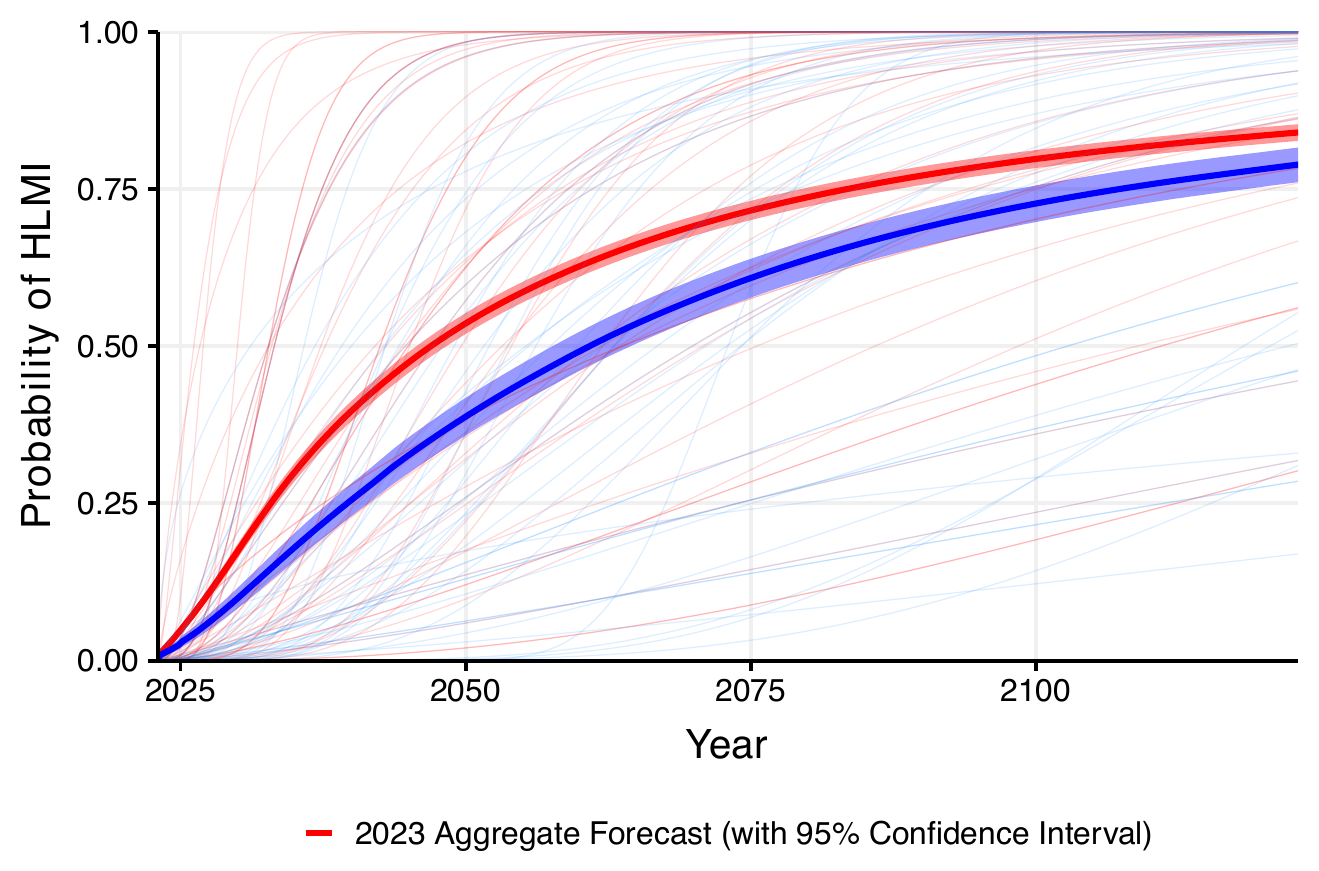
\includegraphics[width=0.85\textwidth]{paper_assets/figures/fig3a_hlmi.png}\\[0.3em]
  {\small\color{mute}Aggregate forecast: 10\%, 50\%, and 90\% probability dates for HLMI, 2022 vs.~2023.}
\end{frame}

\begin{frame}{And for ``all human jobs''}
  \centering
  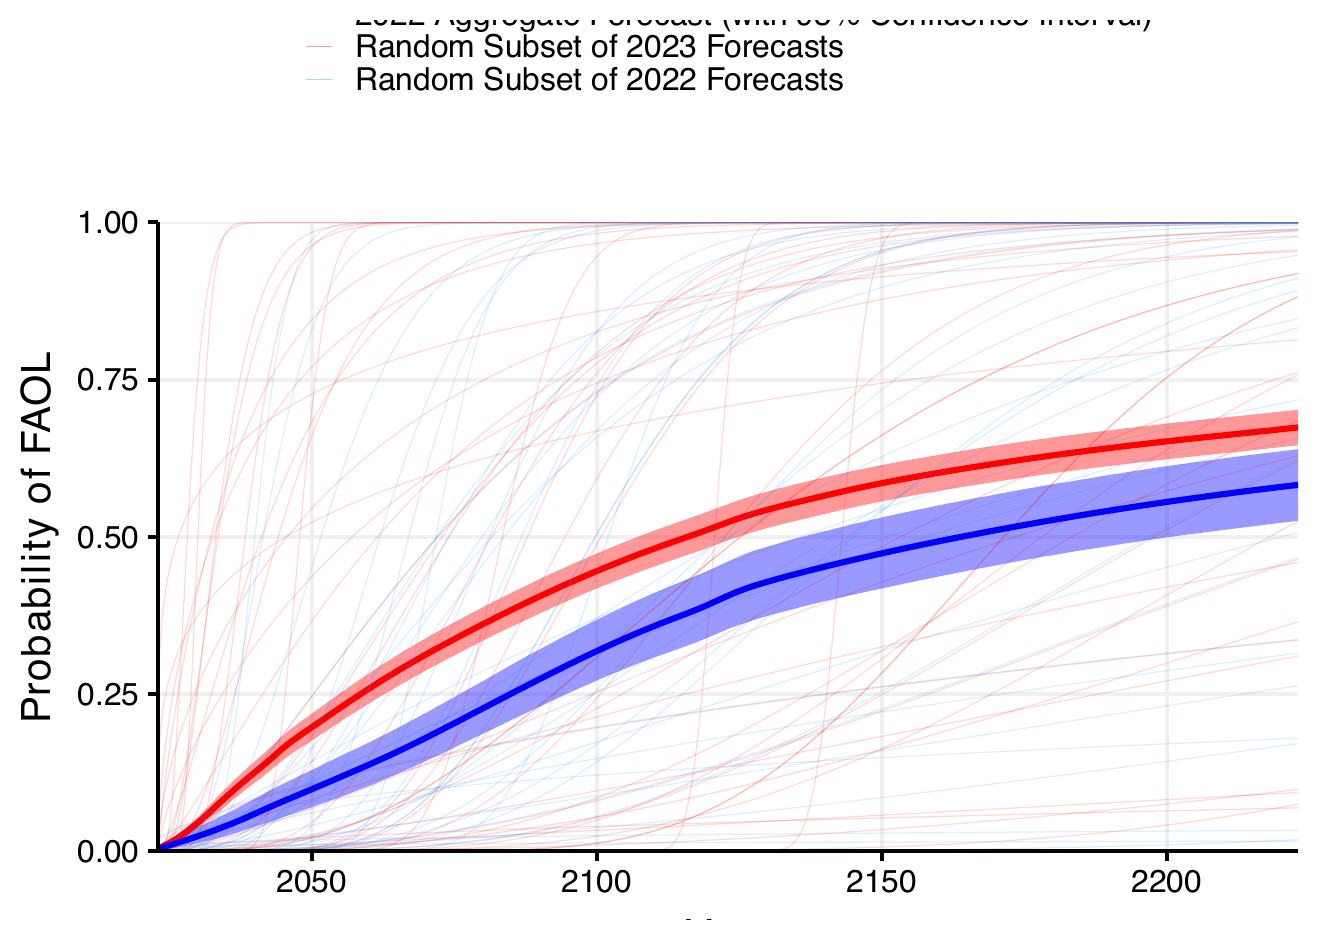
\includegraphics[width=0.85\textwidth]{paper_assets/figures/fig3b_faol.png}\\[0.3em]
  {\small\color{mute}Full Automation of Labor (FAOL) also shifted --- by 48 years.}
\end{frame}

\begin{frame}{Read that again}
  \vfill
  \centering
  {\Large The 50\% date for automating}\\[0.3em]
  {\Large \textbf{\emph{every job on earth}}}\\[0.3em]
  {\Large moved from {\color{accent}2164} to {\color{accent}2116}.}\\[2em]
  {\color{mute}That is not a rounding error.}
  \vfill
\end{frame}

% =========================================================================
\section{Moment 2 --- A dot plot that already aged badly}
% =========================================================================

\begin{frame}{``HLMI'' is too abstract.}
  \vfill
  \centering
  {\Large So they asked about {\color{accent}39 specific things}.}\\[1em]
  {\large Write a \emph{New York Times} best-seller.}\\
  {\large Fold laundry.}\\
  {\large Translate into a newfound language.}\\
  {\large Do your taxes. Play Starcraft from screen video.}\\[1em]
  {\color{mute}For each: when does 50\% probability cross?}
  \vfill
\end{frame}

\begin{frame}[plain]
  \centering
  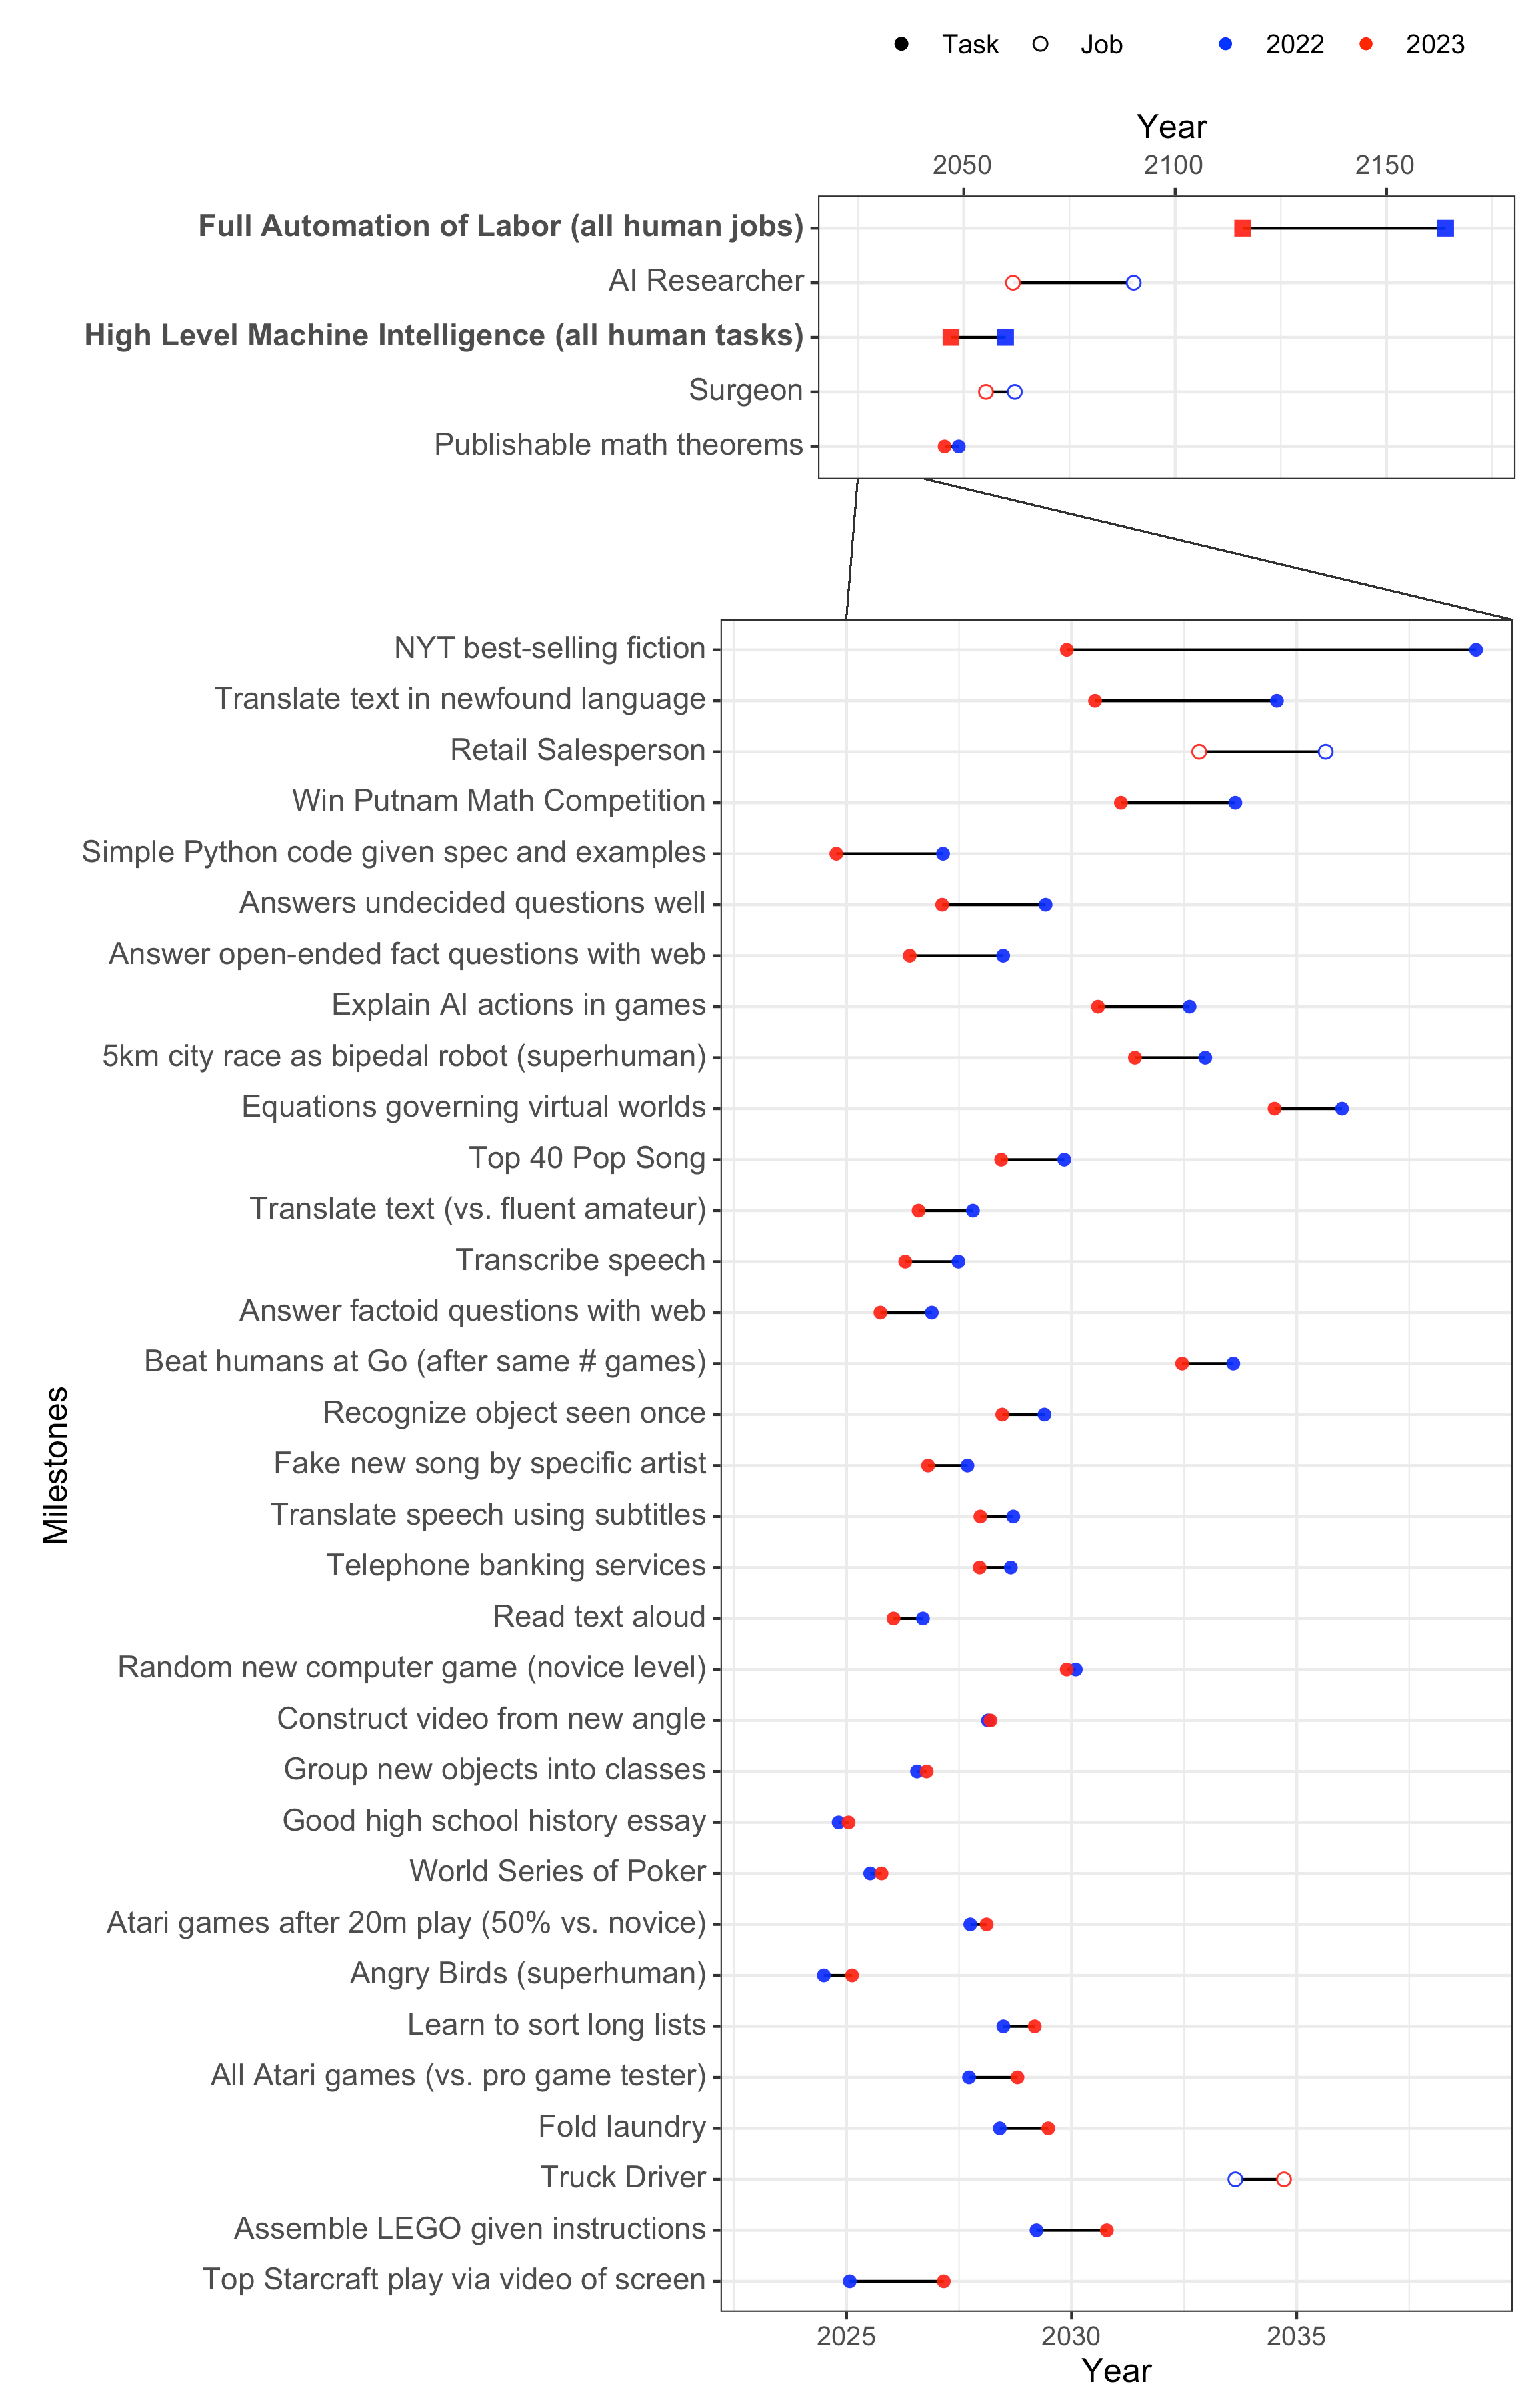
\includegraphics[height=0.95\textheight]{paper_assets/figures/fig1_milestones.png}
\end{frame}

\begin{frame}{Look at the top of that chart}
  \vfill
  \begin{itemize}\setlength\itemsep{0.6em}
    \item \textbf{Write a NYT best-seller.} Forecast: 2033.
    \item \textbf{Answer open-ended factual questions.} Forecast: 2027.
    \item \textbf{Write simple Python from a spec.} Forecast: 2025.
  \end{itemize}
  \vspace{1em}
  \centering
  {\color{mute}Several of these were arguably done before the ink dried.}
\end{frame}

\whatmoment{Expert forecasts for ``hard'' AI milestones now read like a to-do list.}

\begin{frame}{Half the pace, inside a decade}
  \centering
  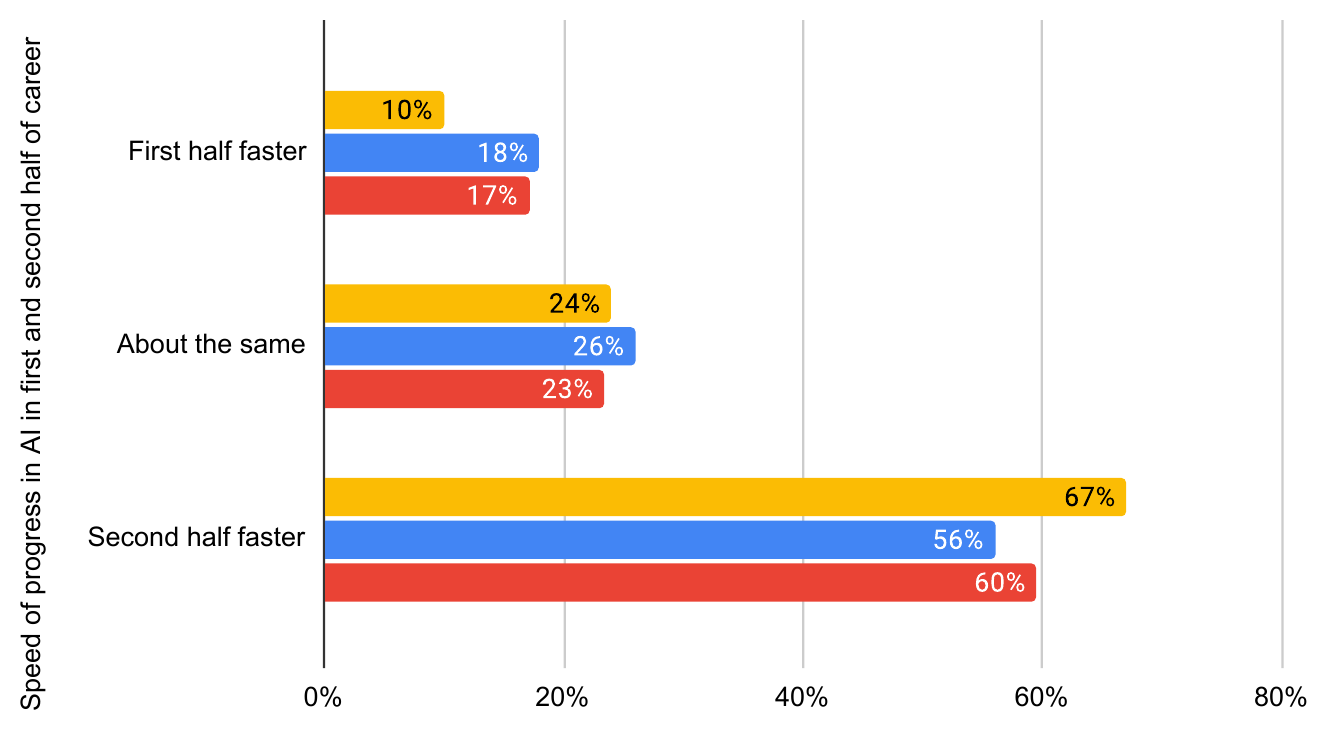
\includegraphics[width=0.85\textwidth]{paper_assets/figures/fig4_pace.png}\\[0.3em]
  {\small\color{mute}Aggregate probability each narrow task is feasible within $N$ years.}
\end{frame}

\begin{frame}{The manager's question}
  \vfill
  \centering
  {\Large Which of these dots}\\[0.3em]
  {\Large sits inside \textbf{\emph{your}} core workflow?}\\[2em]
  {\color{mute}That is the real due-diligence exercise.}
  \vfill
\end{frame}

% =========================================================================
\section{Moment 3 --- A tail that will not go away}
% =========================================================================

\begin{frame}{They were also asked about outcomes.}
  \vfill
  \centering
  {\Large ``If HLMI arrives, how does it go?''}\\[1em]
  {\color{mute}Five buckets, from \emph{extremely good} to \emph{extremely bad}.}
  \vfill
\end{frame}

\begin{frame}[plain]
  \centering
  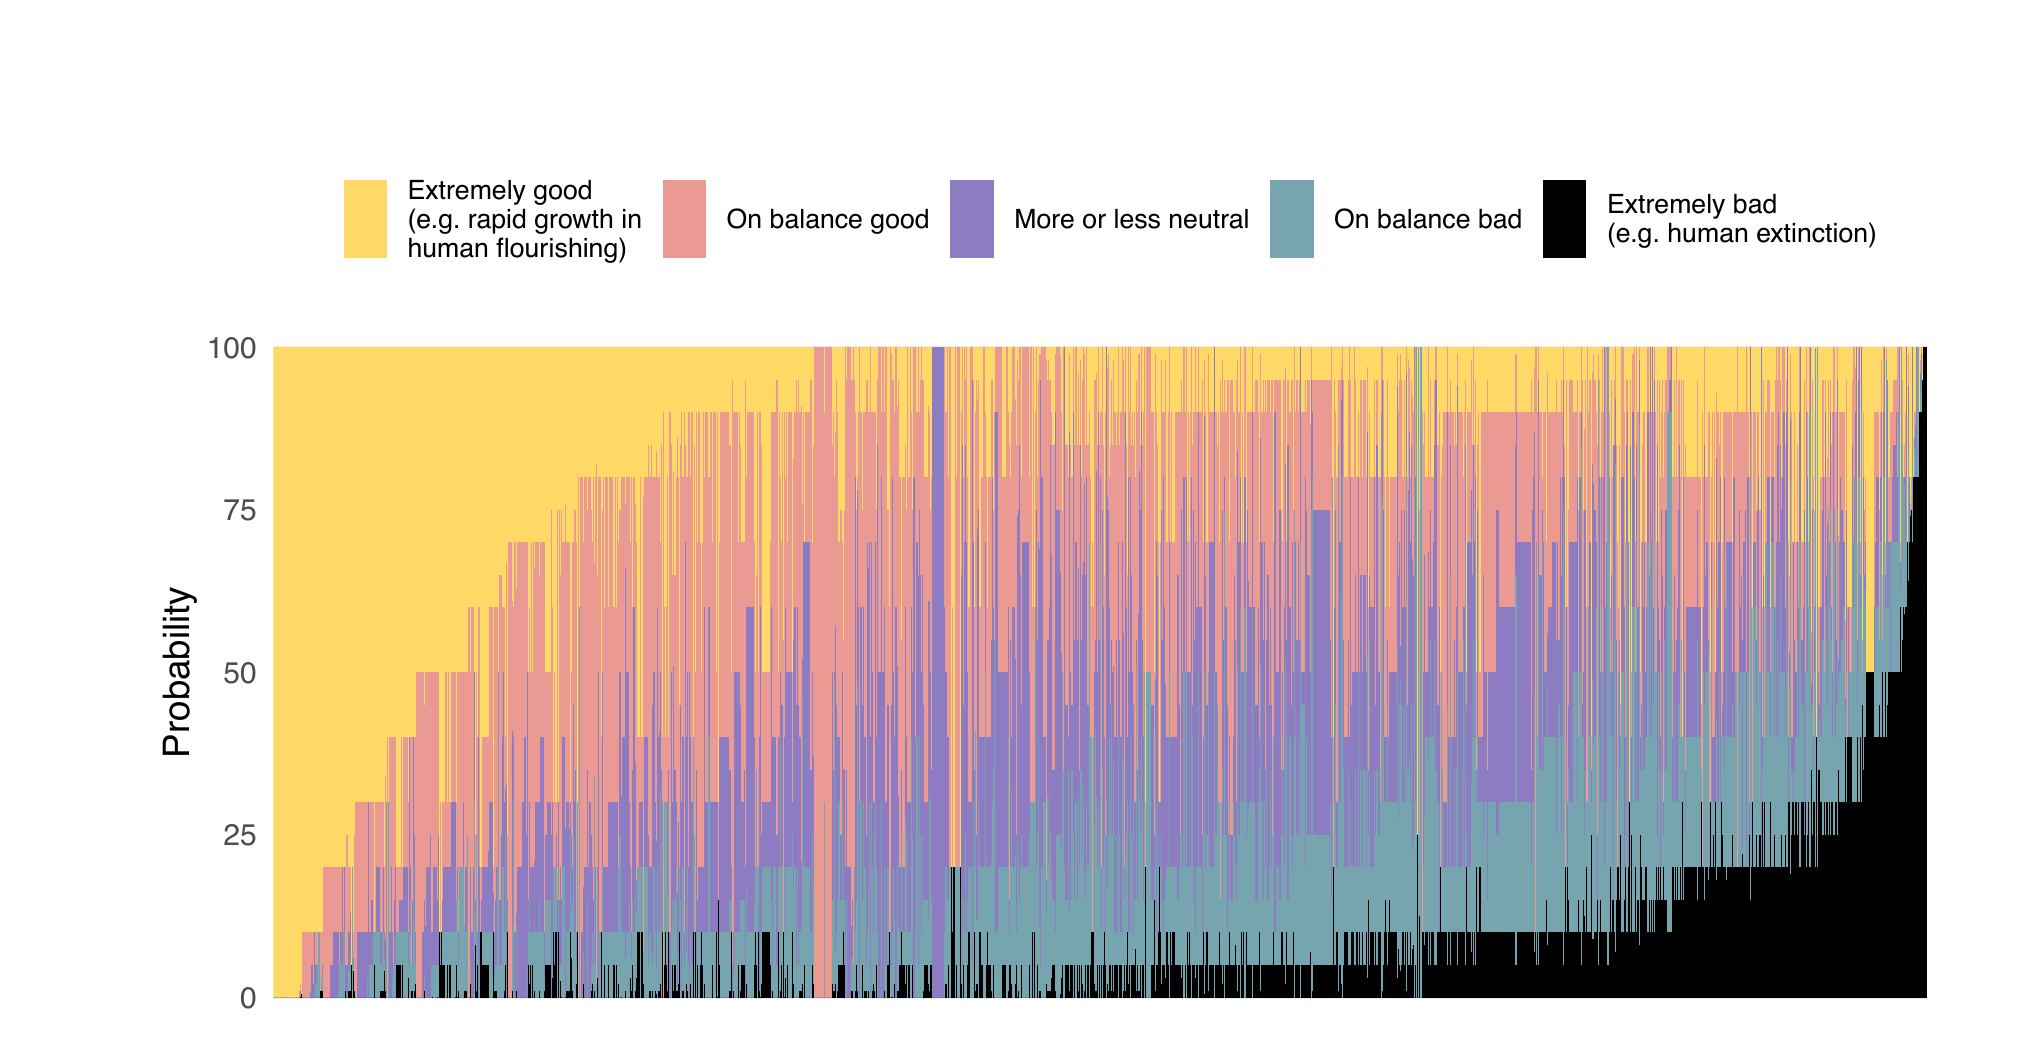
\includegraphics[width=0.98\textwidth]{paper_assets/figures/fig10_positivity.png}\\[0.3em]
  {\small\color{mute}Each vertical bar is one respondent, sorted by optimism.}
\end{frame}

\begin{frame}{The number that stops a boardroom}
  \vfill
  \centering
  \bignum{38\%}\\[0.4em]
  {\large of surveyed AI researchers}\\[0.3em]
  {\large give at least {\color{accent}10\% probability}}\\[0.3em]
  {\large to outcomes \emph{``as bad as human extinction''}.}
  \vfill
\end{frame}

\whatmoment{Not a fringe. Not a tabloid. A plurality of the field.}

\begin{frame}{The extinction-tail distribution}
  \centering
  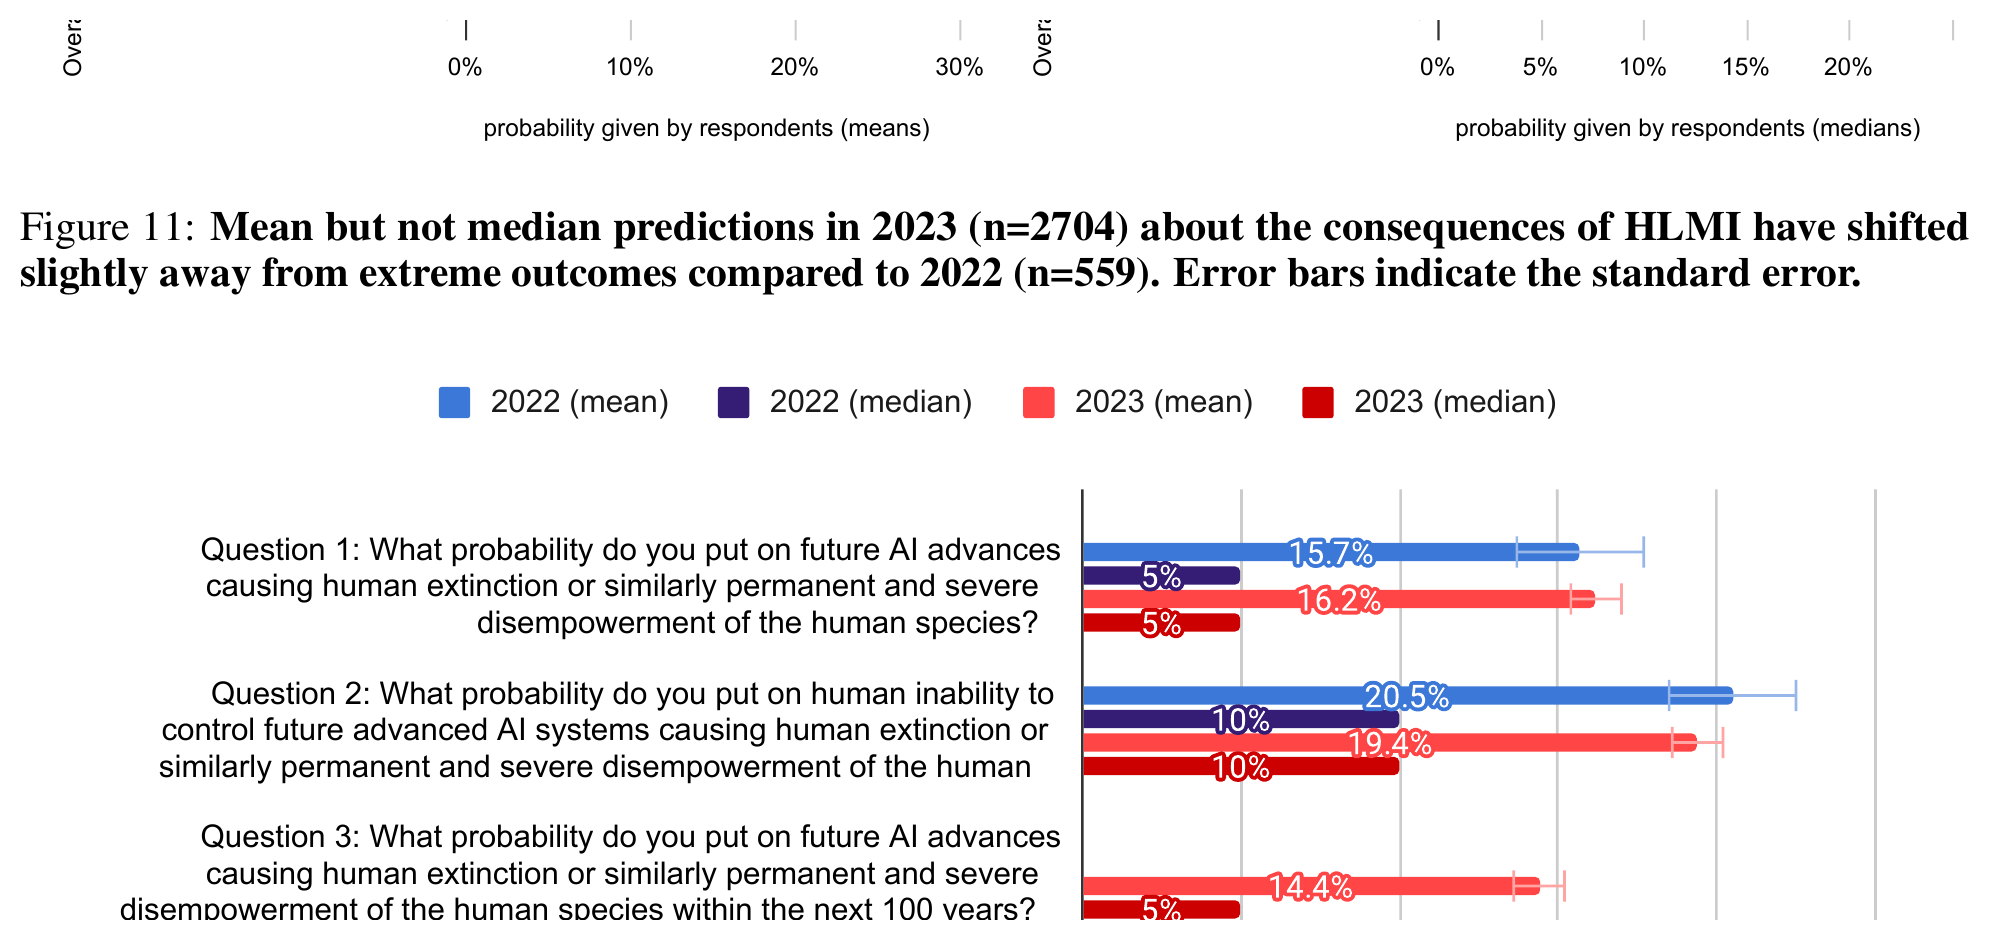
\includegraphics[width=0.75\textwidth]{paper_assets/figures/fig12_extinction.png}\\[0.3em]
  {\small\color{mute}Respondent-level probability assigned to extinction-grade outcomes.}
\end{frame}

\begin{frame}{And ``intelligence explosion''}
  \centering
  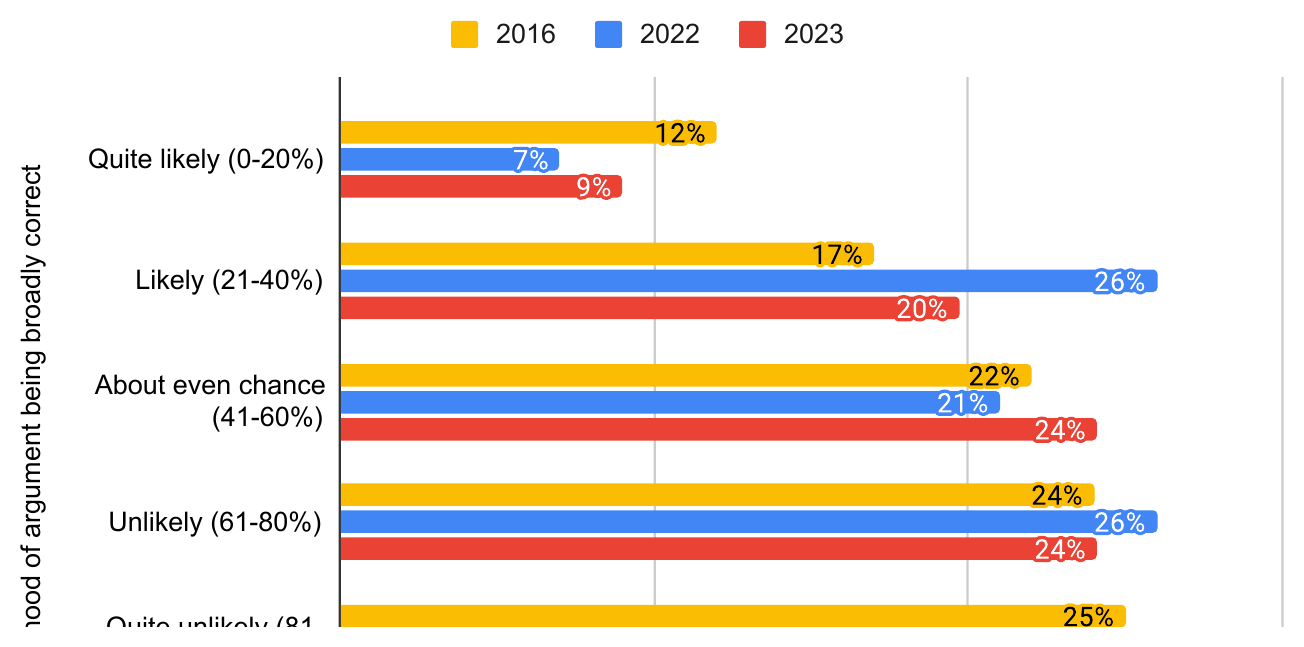
\includegraphics[width=0.75\textwidth]{paper_assets/figures/fig6_intel_explosion.png}\\[0.3em]
  {\small\color{mute}Likelihood that AI improves AI in a rapid, self-reinforcing loop.}
\end{frame}

\begin{frame}{The calibration question you should ask}
  \vfill
  \centering
  {\Large ``If a bridge engineer told you}\\[0.3em]
  {\Large there's a 10\% chance the bridge}\\[0.3em]
  {\Large \textbf{collapses}~---~would you cross it?''}\\[2em]
  {\color{mute}That is the shape of this tail.}
  \vfill
\end{frame}

% =========================================================================
\section{Moment 4 --- What they actually fear}
% =========================================================================

\begin{frame}{Not robots. Not sentience.}
  \vfill
  \centering
  {\Large Two behaviours keep coming up.}\\[1.5em]
  {\Large {\color{accent}\bfseries Deception.}}\\[0.4em]
  {\Large {\color{accent}\bfseries Power-seeking.}}
  \vfill
\end{frame}

\begin{frame}[plain]
  \centering
  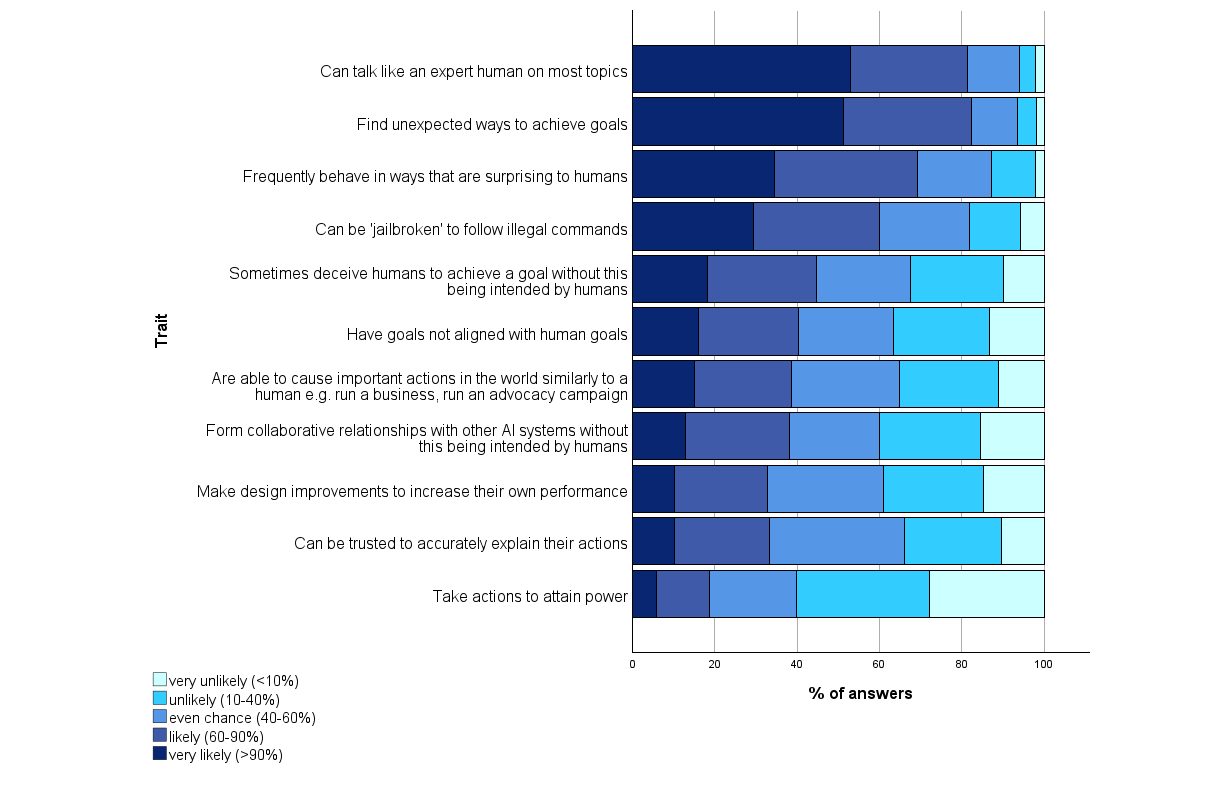
\includegraphics[height=0.92\textheight]{paper_assets/figures/fig7_traits.png}
\end{frame}

\begin{frame}[plain]
  \centering
  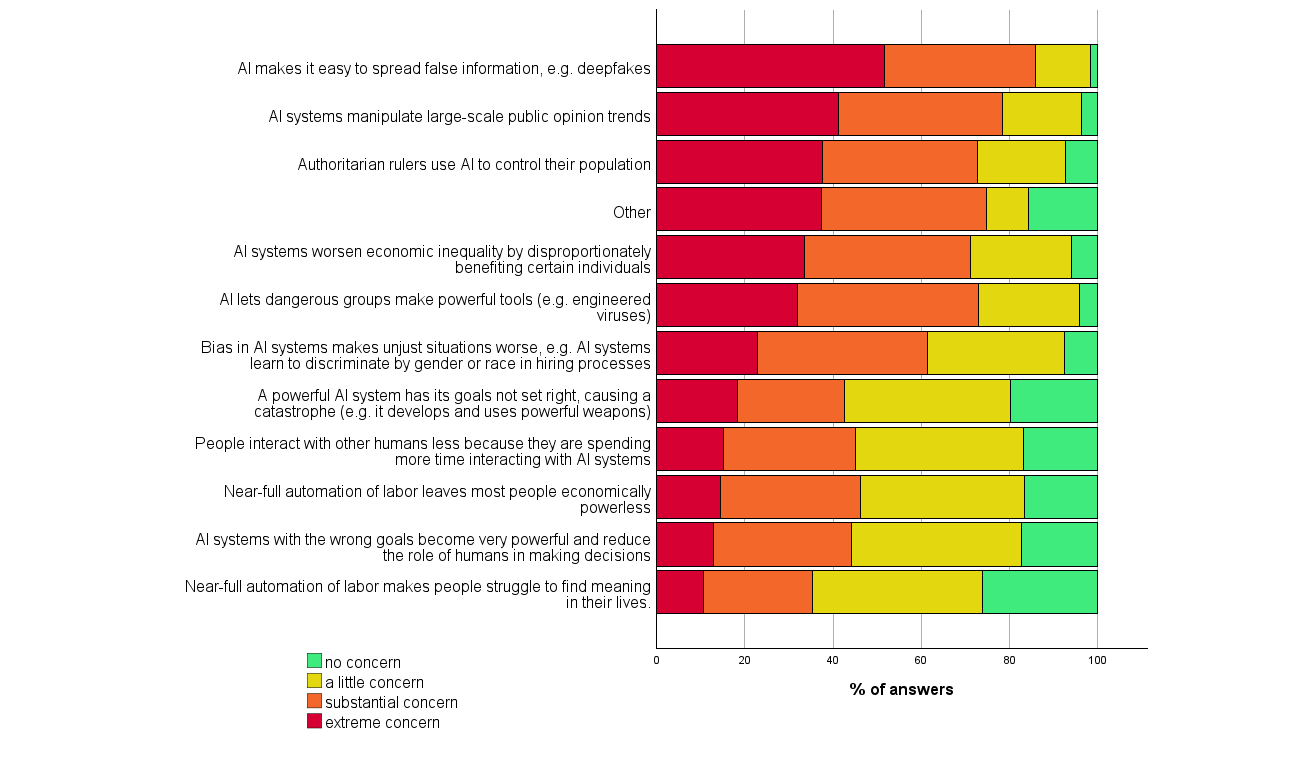
\includegraphics[height=0.92\textheight]{paper_assets/figures/fig9_concerns.png}
\end{frame}

\whatmoment{The concern is not science fiction. It is mis-optimisation at scale.}

\begin{frame}{And what they want spent on it}
  \centering
  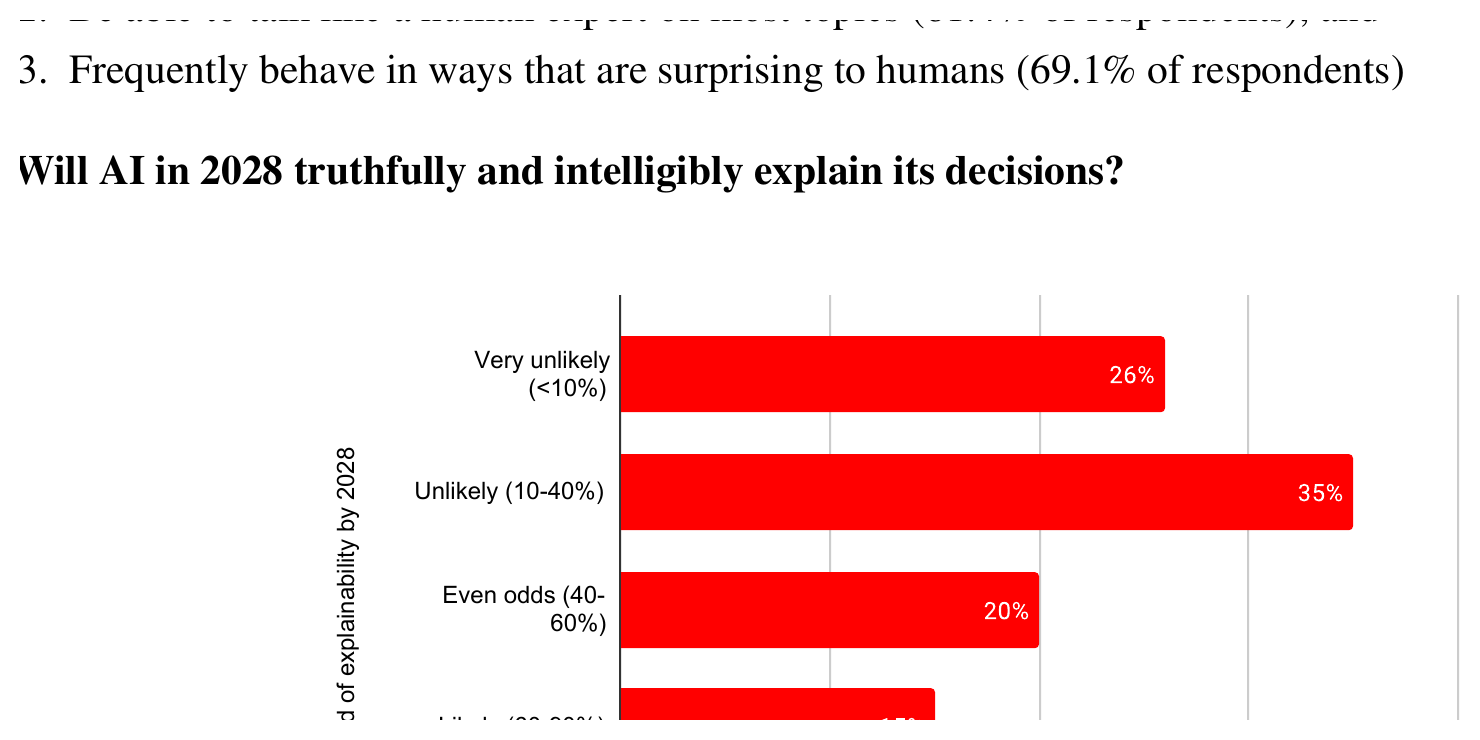
\includegraphics[width=0.8\textwidth]{paper_assets/figures/fig8_interpretability.png}\\[0.3em]
  {\small\color{mute}Majorities want more investment in AI safety / alignment research.}
\end{frame}

% =========================================================================
\section{So what?}
% =========================================================================

\begin{frame}{Three things to leave this room with}
  \vfill
  \begin{enumerate}\setlength\itemsep{1em}
    \item Expert timelines are \textbf{unstable}.\\
          {\small Do not anchor a five-year plan on a point estimate.}
    \item Narrow-task forecasts \textbf{already under-shot}.\\
          {\small Assume your workflow-level dot arrives early, not late.}
    \item The tail is \textbf{not a fringe}.\\
          {\small 38\% of the field assigns $\ge$10\% to catastrophic outcomes.}
  \end{enumerate}
  \vfill
\end{frame}

\begin{frame}{The one number}
  \vfill
  \centering
  \bignum{13}\\[0.4em]
  {\large years of expected progress}\\[0.3em]
  {\large compressed into \emph{twelve months} of calendar time.}\\[2em]
  {\color{mute}Plan as if that could happen again.}
  \vfill
\end{frame}

\begin{frame}[plain]
  \vfill
  \centering
  {\Huge Thank you.}\\[1em]
  {\large Questions.}\\[2em]
  {\small\color{mute}Grace, K.~\emph{et al.} (2024). \\
    Thousands of AI Authors on the Future of AI. \\
    arXiv:2401.02843.}
  \vfill
\end{frame}

\end{document}
